\documentclass[12pt]{article}
 \usepackage{graphicx} 
\usepackage{multirow}
\usepackage{listings}
\usepackage{pythonhighlight}
\usepackage{todonotes}
\usepackage{xcolor}


\begin{document}
\title{Exploration and Presentation - Assignment 3}
\maketitle
\author{
  benjamin kongshaug
  \texttt{cph-bk131@cphbusiness.dk}

}
\author{
  Amanda Hansen
  \texttt{cph-ah433@cphbusiness.dk}

}
\author{
  Amalie Landt
  \texttt{cph-sl307@cphbusiness.dk}

}
\thispagestyle{empty}
\pagebreak

\setcounter{secnumdepth}{4}
\tableofcontents

\pagebreak

\newpage
\section{Introduction}

Vi har fået udleveret projektet LetterFrequencies. Programmet læser indholdet af et dokumentet kaldet FoundationSeries.txt og tæller antallet af hver bogstav i dokumentet. 
Vi har i dette projekt optimeret programmet og dokumenteret analyse af baseline samt de ændringer vi har lavet og hvordan det har forbedret programmet.
\newpage
\section{Task 1}

\subsection{Find a point in your program that can be optimized (for speed), for example by using a profiler}

Før optimering tager programmet: Time elapsed (millisec): 389 \\ \\
Først og fremmest kan vi se 83 procent af tiden befinder programmet sig i metoden tallychars og at det er her vi skal optimere \\ \\
Sekundært ser vi en ligelig fordeling på 33,3 procent af tiden brugt på at lægge input i hashMap og på at læse fra input reader filen \\ \\
Vi kan optimere ved at finde en alternativ måde at indlæse fra filen og ved at gemme mængden af hver bogstav på en mere effektiv måde

\begin{figure}[h!]
\begin{center}
\caption{Output fra profiler}
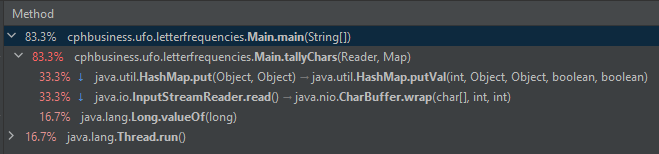
\includegraphics[width=15cm]{før_optimering.PNG}
\label{fig:cclogo}
\end{center}
\label{fig:firstFigureLabel}
\end{figure}




\subsection{A hypothesis of what causes the problem}
Reader reader = new FileReader(fileName);
En reader læser data fra en fil, en linje af gangen når man bruger reader.read() hvilket ikke er særlig effektivt når man har af gøre med en stor fil 

\subsection{A changed program with better performance}
ved at anvende en BufferedInputStream istedet for en reader kan vi gøre indlæsningen af dataen hurtigere, da vores .read metode tager mod data fra bufferen istedet for filen og det er hurtigere at indlæse data fra en buffer. \\ \\

Vi forbedre programmet ved at anvende en Buffered input stream som illustret nedenfor:



\definecolor{codegreen}{rgb}{0,0.6,0}
\definecolor{codegray}{rgb}{0.5,0.5,0.5}
\definecolor{codepurple}{rgb}{0.58,0,0.82}
\definecolor{backcolour}{rgb}{0.95,0.95,0.92}

\lstdefinestyle{mystyle}{
    backgroundcolor=\color{backcolour},   
    commentstyle=\color{codegreen},
    keywordstyle=\color{magenta},
    numberstyle=\tiny\color{codegray},
    stringstyle=\color{codepurple},
    basicstyle=\ttfamily\footnotesize,
    breakatwhitespace=false,         
    breaklines=true,                 
    captionpos=b,                    
    keepspaces=true,                 
    numbers=left,                    
    numbersep=5pt,                  
    showspaces=false,                
    showstringspaces=false,
    showtabs=false,                  
    tabsize=2
}

\lstset{style=mystyle}


\begin{lstlisting}[language=Java, caption=Optimised tallyChars]
String fileName = "/Users/benja/Documents/Downloads/letterfrequencies/src/main/resources/FoundationSeries.txt";
//Reader reader = new FileReader(fileName);

File f = new File(fileName);
FileInputStream fis = new FileInputStream(f);
BufferedInputStream reader = new BufferedInputStream(fis);

\end{lstlisting}


\newpage
\subsection{Make a measurement of the point to optimize, for example by running a number of times, and calculating the mean and standard deviation (see the paper from Sestoft)}

Tid for metoden at køre før optimering i millisec over 100 kørsler :
\\
\\

[394, 394, 394, 394, 394, 394, 395, 395, 395, 395, 397, 397, 397, 397, 397, 397, 397, 397, 397, 397, 397, 397, 397, 398, 398, 398, 398, 398, 398, 398, 398, 398, 398, 398, 398, 398, 398, 398, 398, 398, 399, 399, 399, 399, 399, 399, 399, 399, 399, 399, 399, 399, 399, 399, 399, 399, 399, 399, 399, 399, 399, 399, 399, 402, 402, 402, 402, 402, 402, 405, 405, 405, 405, 405, 405, 405, 405, 405, 405, 405, 405, 405, 405, 405, 405, 405, 405, 405, 405, 405, 405, 405, 405, 406, 406, 406, 406, 407, 407, 407]
\\
\\
Tid for metoden at køre efter optimering i millisec over 100 kørsler:
\\
\\

[202, 202, 202, 202, 202, 202, 202, 202, 202, 202, 202, 202, 202, 202, 202, 202, 202, 202, 202, 202, 202, 202, 202, 202, 202, 202, 202, 202, 202, 202, 202, 202, 202, 202, 202, 202, 202, 202, 202, 202, 202, 202, 202, 202, 202, 202, 202, 202, 202, 202, 202, 202, 203, 203, 203, 203, 203, 203, 203, 203, 203, 203, 203, 203, 203, 203, 203, 203, 203, 203, 203, 203, 203, 203, 203, 203, 203, 203, 203, 203, 203, 203, 203, 203, 203, 203, 203, 203, 203, 203, 203, 203, 203, 203, 203, 203, 203, 203, 203, 203]
\\
\\

\begin{figure}[h!]
\begin{center}
\caption{box plots af proformance}
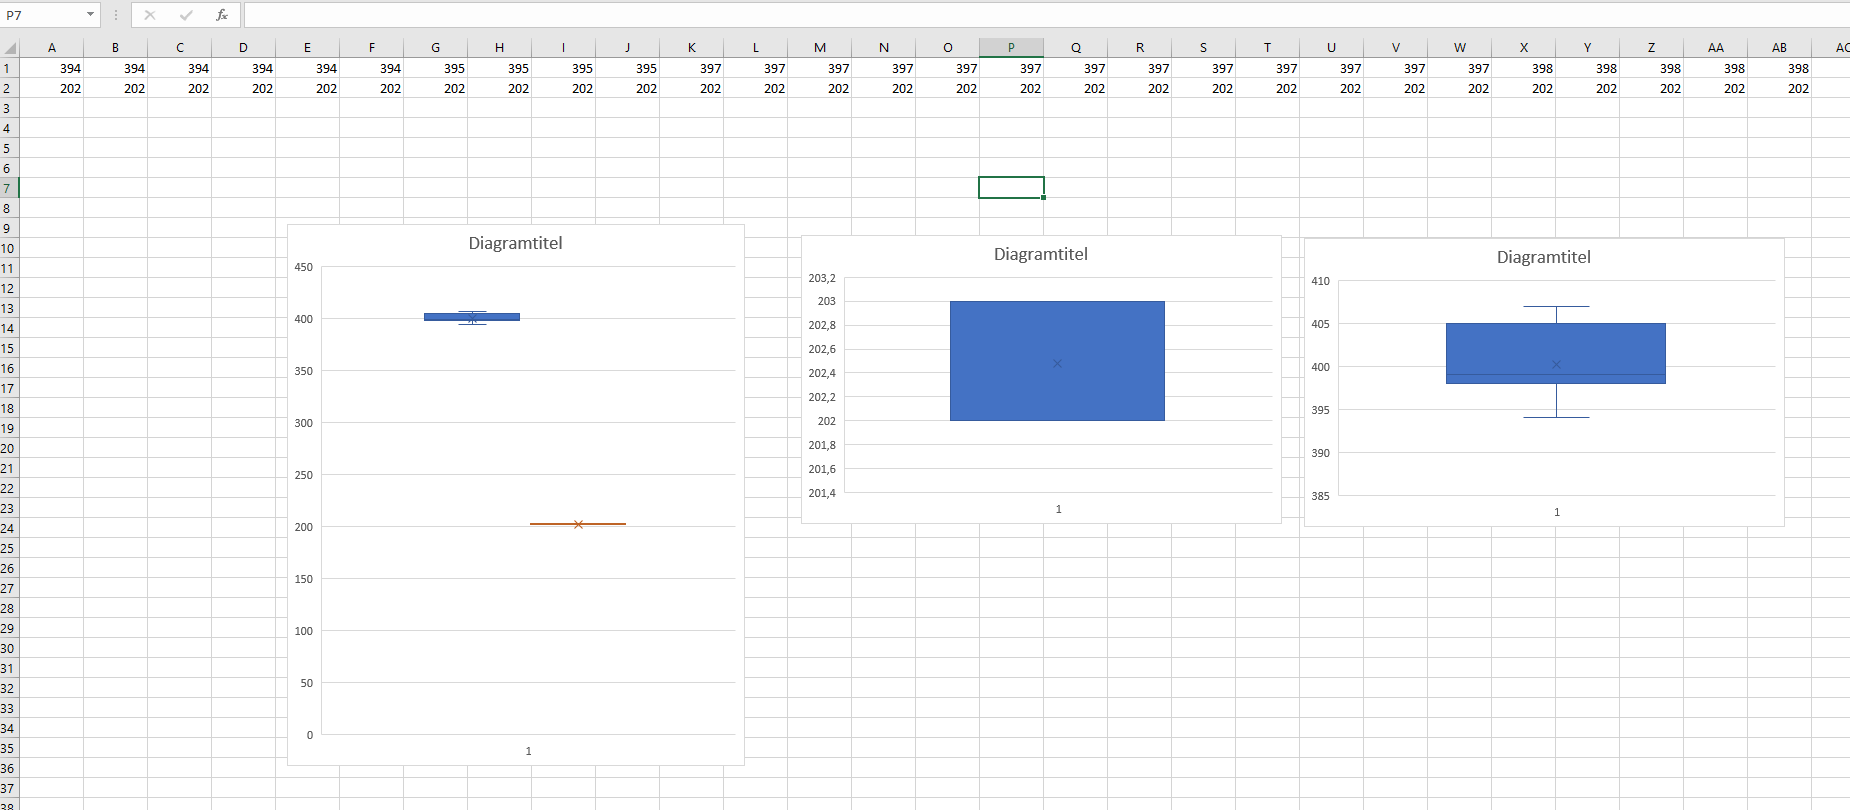
\includegraphics[width=15cm]{box plot.PNG}
\label{fig:cclogo}
\end{center}
\label{fig:firstFigureLabel}
\end{figure}





Vi kan se ud fra vores box plot at vores mean og standard diviacion på ingen måde overlapper og at der tydeligt er et proformance boost i vores program.  \\

\newpage
\section{Conclusion}
Vi har ved at anvede en profiler fundet frem til at programmet bruger 33 procent af runtime på at læse fra filen, som anvender en FileReader. Vi har optimeret ved at udskifte FileReaderen med en BufferedInputStream. Før optimering var vores average performance omkring 400 milisec og den ligger nu omkring 200 milisec. Vi har derfor opnået en 50 procents forbedring.



\end{document}
